\documentclass[12pt,a4paper]{article}

\usepackage{setspace}
\onehalfspacing
\usepackage{caption}
\usepackage{subcaption}
\usepackage{float}
\captionsetup[table]{font={stretch=1.5}}     %% change 1.5 as you like
\captionsetup[figure]{font=onehalfspacing}    %% change onehalfspacing as you like
\usepackage[english]{babel}
\usepackage[utf8]{inputenc}
\usepackage{amsmath}
\usepackage{amssymb}
\usepackage{graphicx}
\usepackage[colorinlistoftodos]{todonotes}
\usepackage[top=0.75in,left=0.75in,right=0.75in,bottom=0.75in]{geometry}
\usepackage{multicol,caption}
\usepackage{makeidx}
\usepackage{pdfpages}
\usepackage[compat=1.0.0]{tikz-feynman}
\usepackage{hyperref}
%\usepackage{LuaLaTeX}
\makeindex
%\usepackage{fixltx2e}
\usepackage{cite}
\newenvironment{Figure}
  {\par\medskip\noindent\minipage{\linewidth}}
  {\endminipage\par\medskip}
\setlength{\columnsep}{1cm}
\setlength{\parindent}{0pt}
\usepackage{color,soul}
\usepackage{booktabs}
\newcommand{\ra}[1]{\renewcommand{\arraystretch}{#1}}

\title{Overview and Literature survey}
\date{\today}
\author{Ronald Collins ID:200948843}

\begin{document}
\maketitle

\begin{Figure}
 \centering
 
\includegraphics[width=1.0\linewidth]{Liverpool_logo}
 \captionof*{figure}{} 
\end{Figure}


\begin{center}
\textit{Department of Physics, High Energy Physics\\}
\textit{VIDARR collaboration\\}
\end{center}


\pagenumbering{gobble}
\newpage
\pagenumbering{roman}
\begin{abstract}
\normalsize A basic overview\\

\providecommand{\keywords}[1]{\textbf{\textit{Keywords:}} #1} %Keywords command has to be supplied manually
\keywords{Monte Carlo, Geant4, High performance computing (HPC), Anti-neutrino}
\end{abstract}
\vspace{5mm} %5mm vertical space before main body of text
%\begin{multicols}{2}
\tableofcontents
\newpage

\pagenumbering{arabic}

\section{Discovery of neutrinos}
\subsection{Theoretical Development}
history of neutrino: \cite{griffiths2008introduction} \cite{lederman1970resource}
\\beta decay of tritium (book cannot find, may have to replicate): \cite{lewis1970neutrinos} especially as Fermi mentions it in \cite{Fermi:1934hr}, \cite{wilson1968fermi} 
\\Neutron proposed by Chadwick in 1932 describing a proton like recoil and odd behaviour of neutrons that can only be described by a neutron or the breaking of conservation of momentum and energy!: \cite{chadwick1932possible}. Important for giving full context to the neutrino discovery
\\Fermis paper proposing this beta decay after Chadwick's discovery of the neutron is given in \cite{Fermi:1934hr} which proposes a neutrino and is published through Springer and the English translation from 1968 is given in \cite{wilson1968fermi}
\\So far very little from Pauli need to include him somewhere the neutrino was his idea \cite{lederman1970resource} may have something...

\begin{Figure}
 \centering
 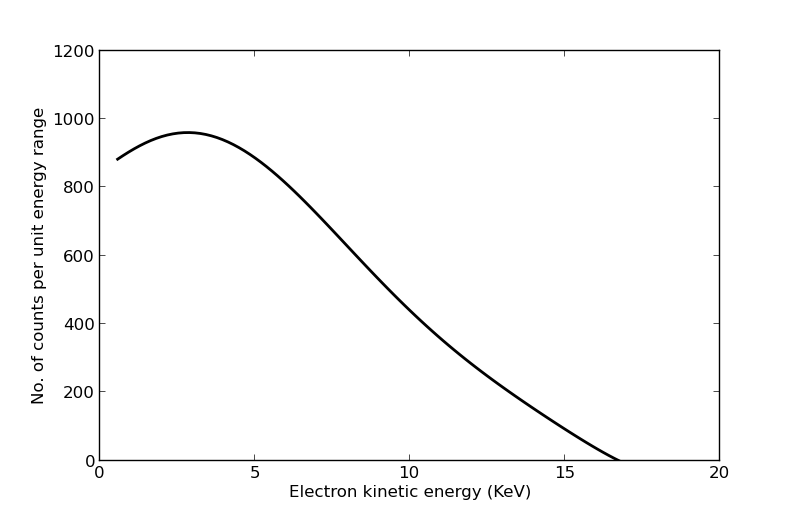
\includegraphics[height=90mm]{beta_spectrum.png}
 \captionof{figure}{beta spectrum from \cite{griffiths2008introduction} originally from \cite{lewis1970neutrinos}, the energies of the beta particle vary significantly, which would not occur without another particle being involved with beta decay} %~can be used as a kind of place holder in latex
 \label{beta_spectrum}
\end{Figure}

\subsection{Direct Measurements}
propossal of cowan and riens using a large liquid scintillator detector: \cite{reines1953proposed}
\\First detection: \cite{reines1953detection}
\\distingiusing the neutrino and anti-neutrino \cite{davis1959attempt}
\\Need to find cloud chamber pictures showing the conservation of momentum \cite{griffiths2008introduction} shows them, need to find direct source. \cite{griffiths2008introduction} also goes on to explain why this matters.
\\ \cite{michel1949energy} supposedly does show this, but I'm having trouble getting my hands on it, UoL doesn't have access to nature papers! So will just have to include a picture from \cite{griffiths2008introduction} and clarifiy it is from \cite{michel1949energy}.
\\ There is also the suggestion from cowan early on that anti-neutrinos and neutrinos are differing particles,  \cite{cowan1957test}, however this is by no means certain it is possible that neutrinos and anti-neutrinos are differing spin states of the same particle.
\\ There is also the early suggestion of neutrinos and anti neutrinos being separated by a certain quantity suggested by \cite{konopinski1953universal} under a universal interaction. They use muons to suggest that certain reactions are not possible, this would later come to be known as lepton number. \\\\


\begin{Figure}
 \centering
 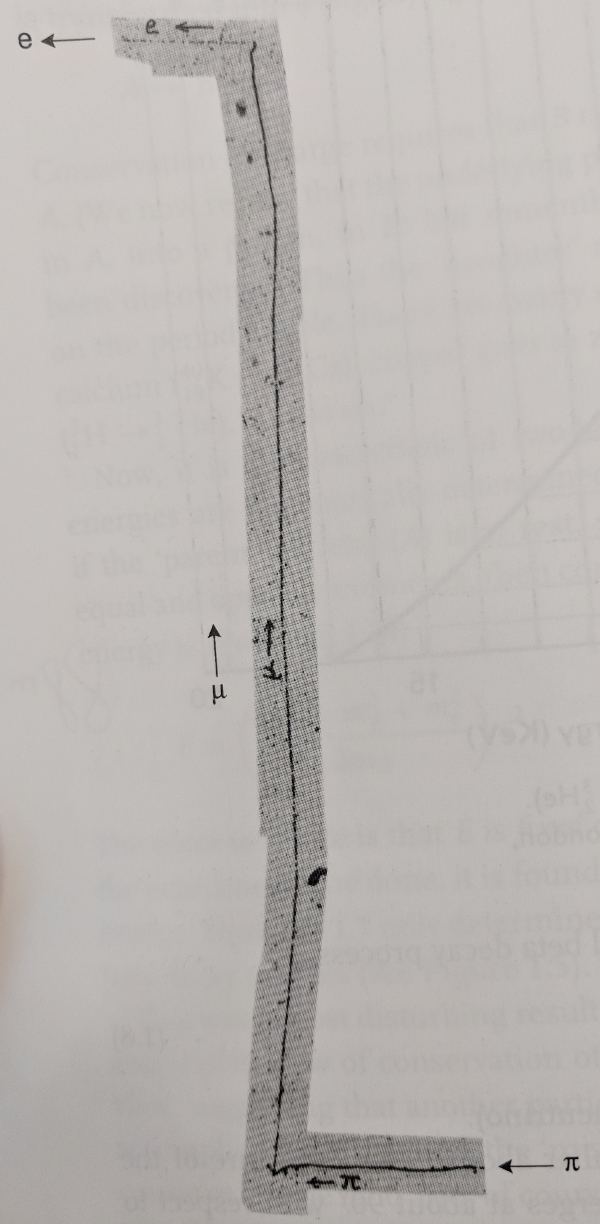
\includegraphics[height=90mm]{less_detailed_path.jpg}
 \captionof{figure}{Path of pion decaying to a muon emitting one anti-neutrino and then that muon decaying into an electron emitting a neutrino and an anti-neutrino. The paths at 90$^o$ show particle decay, collisions cannot account for this. From \cite{griffiths2008introduction} originally from \cite{michel1949energy}.} %~can be used as a kind of place holder in latex
 \label{beta_spectrum}
\end{Figure}

\section{Anti-neutrino Reactor Monitoring}
\subsection{Anti-neutrino Production}
\subsection{Anti-neutrino Detection}

\section{Solar Neutrinos}

\section{Neutrino Flavours}
\subsection{Neutrino oscillations}
\subsection{Mixing Angles}

\section{Existing Reactor monitoring programs}

\bibliography{refs} 
\bibliographystyle{ieeetr}

\end{document}
